\documentclass{article}
\usepackage[a4paper,margin=20mm]{geometry}
\usepackage[T1]{fontenc}
\usepackage{lmodern}

\usepackage{microtype}
\usepackage{graphicx}
\graphicspath{{../figures/}{figures/}}
\usepackage{subcaption}
\usepackage{booktabs}
\usepackage{float}
\usepackage{balance}

\usepackage{hyperref}




\usepackage{amsmath}
\usepackage{amssymb}
\usepackage{mathtools}
\usepackage{amsthm}

\usepackage[capitalize,noabbrev]{cleveref}
\DeclareMathOperator{\RN}{RMSNorm}
\DeclareMathOperator{\LN}{LayerNorm}
\DeclareMathOperator{\SiLU}{SiLU}
\setlength{\columnsep}{6mm}
\setcounter{dbltopnumber}{2}
\renewcommand{\dbltopfraction}{0.85}
\renewcommand{\textfraction}{0.1}
\raggedbottom

\title{Analysis and comparison }
\author{}
\date{}

\begin{document}
\twocolumn[\maketitle]


\section{Introduction}
\label{sec:introduction}

Electroencephalography (EEG) provides a noninvasive measurement of brain
electrical activity with high temporal resolution. Learning representations
that transfer across tasks, participants, and recording conditions is a
central objective for EEG foundation models. Recent approaches, including
LaBraM, CBraMod, EEGPT, and REVE, use large-scale self-supervised pretraining
to reduce dependence on task-specific annotations and support multiple
downstream applications~\cite{jiang2024labram,wang2025cbramod,wang2024eegpt,elouahidi2025reve}.
Their evaluation also benefits from established supervised baselines such
as EEGNet, a compact convolutional architecture rather than a pretrained
foundation model~\cite{lawhern2018eegnet}.

Strong decoding performance, however, does not by itself establish which
properties of a recording support a prediction. EEG representations may
encode task-related neural activity alongside participant identity,
session characteristics, acquisition settings, and physiological or
instrumental artifacts. These factors can become predictive when they
correlate with the target labels. Recent diagnostic work reports substantial
subject-related structure in several foundation models, while broader
evaluations reveal model-dependent robustness to noise and channel
loss~\cite{lin2026identity,sirca2026beyond}. Subject information is not
necessarily an artifact: it may also reflect meaningful individual
physiology. Nevertheless, these findings motivate examining what a
representation preserves, beyond its downstream accuracy.

Our exploratory inspections of latent spaces across several EEG datasets
motivate a closer investigation of this issue. In particular, the
four-class motor-imagery task in BCI Competition IV dataset 2a provides
a concrete setting in which to examine whether class separation reflects
motor-related activity or correlated nuisance signals. The dataset includes
electrooculographic recordings and expert artifact annotations, which can
support controlled analyses~\cite{brunner2008bci2a}. Apparent separation in
a latent-space visualization is insufficient to conclude that a model
relies on artifacts, or that it fails to encode useful neural information.
We therefore treat artifact dependence as a hypothesis to test through
targeted controls and ablations, rather than as an established property of
all EEG foundation models.

The pretraining objective is one possible source of differences in the
information retained by an encoder. Existing methods do not all optimize
the same reconstruction target: CBraMod and REVE reconstruct masked EEG
inputs, LaBraM predicts discrete neural codes derived from a learned
tokenizer, and EEGPT already incorporates alignment between learned
representations~\cite{wang2025cbramod,elouahidi2025reve,jiang2024labram,wang2024eegpt}.
Reconstructing a waveform can encourage the preservation of any component
that contributes to reconstruction error, including nuisance variation.
This does not imply that signal-space learning is intrinsically
uninformative, nor that a latent-space objective automatically removes
artifacts. It instead raises the question of how the learning target and
the construction of training views jointly influence the resulting
representation.

Spatial organization provides a complementary inductive bias. Electrode
locations constrain how measurements relate across the scalp, and recent
models explicitly incorporate spatial structure through dedicated mixing
mechanisms or positional information~\cite{wang2025cbramod,elouahidi2025reve}.
At the same time, channel availability, electrode configuration, and
reference choice alter the observations presented to a model. Montage
effects must therefore be separated from differences in architecture and
pretraining objective. Controlled montage ablations can help determine
whether a model benefits from meaningful spatial relationships or remains
dependent on a particular acquisition configuration. Incorporating
electrode geometry alone does not establish invariance to these changes.

Joint-embedding learning offers a way to investigate an alternative to
direct waveform reconstruction. LeJEPA combines agreement between views of
the same sample with a regularizer that encourages an isotropic Gaussian
embedding distribution, providing a mechanism to oppose representation
collapse~\cite{balestriero2025lejepa}. Its recent video extension, LeVJEPA,
also investigates this principle for temporally structured
data~\cite{kuhn2026levjepa}. For EEG, views spanning different temporal
contexts may encourage shared recording-level representations. However,
their usefulness depends on which information the views share: persistent
nuisance factors can also satisfy an agreement objective. The suitability
of this approach for EEG therefore requires empirical evaluation.

We introduce EEGFM, a hierarchical encoder
that combines electrode-wise tokenization, spatial mixing, bidirectional
Mamba processing, and convolutional temporal modeling. Distance-dependent
attention biases encode electrode geometry, and a learned-query bottleneck
aggregates the encoded tokens into a global representation. We train this
representation with a LeJEPA-inspired objective over global and local
temporal views, without a waveform reconstruction loss. The study is
organized around three objectives: characterizing task and nuisance
information in existing representations, isolating montage effects through
controlled ablations, and evaluating the contribution of spatial modeling
and latent-space training in EEGFM.

\section{Related Work}

\section{Methodology}
\label{sec:methodology}

We develop EEGFM, a hierarchical EEG encoder that combines electrode-wise
signal tokenization, spatial mixing, and bidirectional temporal processing.
The model produces both channel-resolved token embeddings and a global
representation of each recording window. We train the global representation
using a multiview objective inspired by LeJEPA~\cite{balestriero2025lejepa},
combining agreement between views with a distributional regularizer.
The following formulation describes the patch-based configuration used in
this work.

Let $X\in\mathbb{R}^{B\times C\times T}$ denote a batch of EEG windows, where
$B$ is the batch size, $C$ the number of channels in a fixed canonical order,
and $T$ the number of time samples. Electrode coordinates are denoted by
$P=(p_1,\ldots,p_C)^\top\in\mathbb{R}^{C\times3}$.
A presence code $a_{bc}\in\{0,1,2\}$ accompanies each channel; code zero marks
an absent channel, and both nonzero codes are treated as available by the
attention masks. We write $m_{bc}=\mathbb{1}[a_{bc}\ne0]$ and assume that each
window contains at least one available channel. Hereafter, $\Vert$ denotes
concatenation, $\odot$ element-wise multiplication, and $\RN$ and $\LN$
denote root-mean-square normalization and layer normalization, respectively.
Features are column vectors, and linear maps act on their last dimension.
The presence input is labeled $p$ in the figures and $a$ in the text.

\subsection{Model Pipeline Overview}
\label{sec:model-overview}

\begin{figure*}[t]
    \centering
    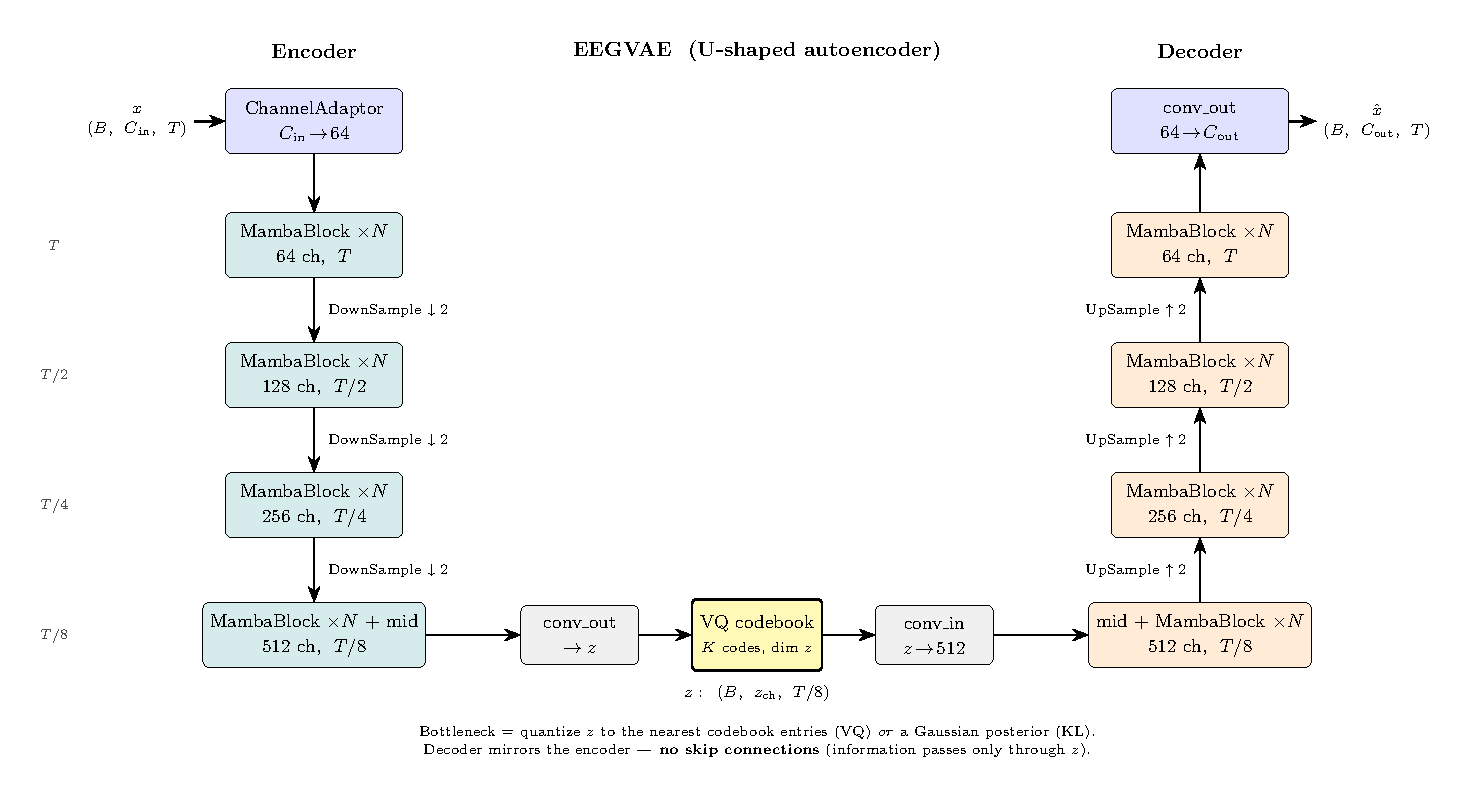
\includegraphics[width=\textwidth]{model_pipeline/model_pipeline.pdf}
    \caption{EEGFM architecture. A patch stem feeds four encoder stages with
    progressively shorter temporal sequences and larger feature dimensions.
    Geodesic distances between electrode coordinates are quantized into
    16 bins and mapped to learned attention biases in the last two stages.
    The bottleneck returns token embeddings $z$ and a global embedding
    $z_{\mathrm{glob}}$ obtained with four learned queries. The input has shape
    $B\times C\times T$; stage lengths are
    $N_i=\lfloor T/(20\cdot2^{i-1})\rfloor$ for $i=1,\ldots,4$.
    Feature widths correspond to the configured encoder.}
    \label{fig:model-pipeline}
\end{figure*}

\Cref{fig:model-pipeline} summarizes the mapping
\begin{equation}
    (Z,g)=f_\theta(X,a;P),
    \label{eq:model-mapping}
\end{equation}
where $Z\in\mathbb{R}^{B\times C\times N_4\times D_z}$ contains the token
embeddings and $g\in\mathbb{R}^{B\times D_z}$ contains the global embeddings.
These correspond to the outputs $z$ and $z_{\mathrm{glob}}$ in the figures.
The channel axis is preserved throughout the encoder; only temporal
resolution and feature dimension change. The input length $T$ is variable;
the configured encoder uses $D_z=384$. At a sampling rate of 200\,Hz,
an input window spans $T/200$ seconds.

\paragraph{Signal tokenization.}
The stem first applies a signed logarithmic compression,
\begin{equation}
    \widetilde X=\operatorname{sign}(X)\odot\log(1+|X|).
    \label{eq:signed-log}
\end{equation}
Each channel is processed independently by the same two temporal convolutional
layers. Both have kernel size nine and are followed by eight-group GroupNorm
and SiLU. The first convolution maps one input feature to $d_s=32$ features;
the second preserves this width and uses eight convolution groups.
Padding preserves the time dimension. The resulting features are partitioned
into non-overlapping patches of $p=20$ samples. With
$N_1=\lfloor T/p\rfloor$, the flattened patch vector
$r_{bcn}\in\mathbb{R}^{pd_s}$ is embedded as
\begin{equation}
    H^{(0)}_{bcn}
    =W_{\mathrm{stem}}\LN(r_{bcn})+e_c+e_{a_{bc}},
    \label{eq:patch-embedding}
\end{equation}
where $W_{\mathrm{stem}}\in\mathbb{R}^{128\times640}$, $e_c$ is a learned
channel embedding, and $e_{a_{bc}}$ is a learned presence embedding.
Any incomplete final patch is discarded.

\paragraph{Hierarchical encoding.}
The four stages use feature widths
$(D_1,D_2,D_3,D_4)=(128,192,256,384)$ and block counts
$(L_1,L_2,L_3,L_4)=(2,2,3,3)$. Between stages, adjacent tokens are concatenated,
normalized, and projected:
\begin{align}
    r^{(i)}_{bcn}
      &=H^{(i)}_{bc,2n-1}\Vert H^{(i)}_{bc,2n},\\
    H^{(i+1,\mathrm{in})}_{bcn}
      &=W_{\downarrow}^{(i)}\RN(r^{(i)}_{bcn}),
    \label{eq:downsampling}
\end{align}
where $W_{\downarrow}^{(i)}\in\mathbb{R}^{D_{i+1}\times2D_i}$ and
$n=1,\ldots,\lfloor N_i/2\rfloor$. An unpaired final token is discarded.
Thus, for patch size $p=20$, the temporal lengths satisfy
\begin{equation}
    N_i=\left\lfloor\frac{T}{p\,2^{i-1}}\right\rfloor,
    \qquad i=1,\ldots,4.
    \label{eq:stage-lengths}
\end{equation}
In particular, $N_4=\lfloor T/160\rfloor$; we require $T\geq160$ so that
at least one temporal token reaches the bottleneck.

\paragraph{Token bottleneck and global readout.}
The final hidden tensor is normalized and optionally projected:
\begin{equation}
    Z_{bcn}=W_z\RN(H^{(4)}_{bcn}).
    \label{eq:token-bottleneck}
\end{equation}
Here $W_z$ is the identity because $D_z=D_4$; a learned projection is used
when these dimensions differ. To obtain $g_b$, the $C N_4$ tokens are
flattened into a sequence $(z_{bj})_j$. For each of $A=8$ attention heads,
linear maps produce keys and values of width $d_z=D_z/A=48$:
\begin{equation}
    k_{bhj}=\RN(W_h^Kz_{bj}),\qquad
    v_{bhj}=W_h^Vz_{bj}.
\end{equation}
Each head has $Q=4$ learned queries $q_{hq}\in\mathbb{R}^{d_z}$. A token
inherits the availability of its channel, denoted by $m_{bj}$. The pooled
head outputs are
\begin{align}
    \alpha_{bhqj}
      &=\frac{m_{bj}\exp(q_{hq}^{\top}k_{bhj}/\sqrt{d_z})}
      {\sum_r m_{br}\exp(q_{hq}^{\top}k_{bhr}/\sqrt{d_z})},\\
    o_{bhq}&=\sum_j\alpha_{bhqj}v_{bhj}.
    \label{eq:global-attention}
\end{align}
Concatenating the heads for each query and then the queries gives
$o_b\in\mathbb{R}^{QD_z}$. The global representation is
\begin{equation}
    g_b=W_{\mathrm{out}}W_{\mathrm{merge}}\RN(o_b),
    \label{eq:global-embedding}
\end{equation}
with $W_{\mathrm{merge}}\in\mathbb{R}^{D_z\times QD_z}$ and
$W_{\mathrm{out}}\in\mathbb{R}^{D_z\times D_z}$. Thus, the global readout
aggregates both channel and temporal information while excluding unavailable
channels as attention keys. Training uses $g_b$ directly; the token output
$Z$ remains available for downstream analysis.

\subsection{Encoder Architecture}
\label{sec:encoder}

\begin{figure*}[t]
    \centering
    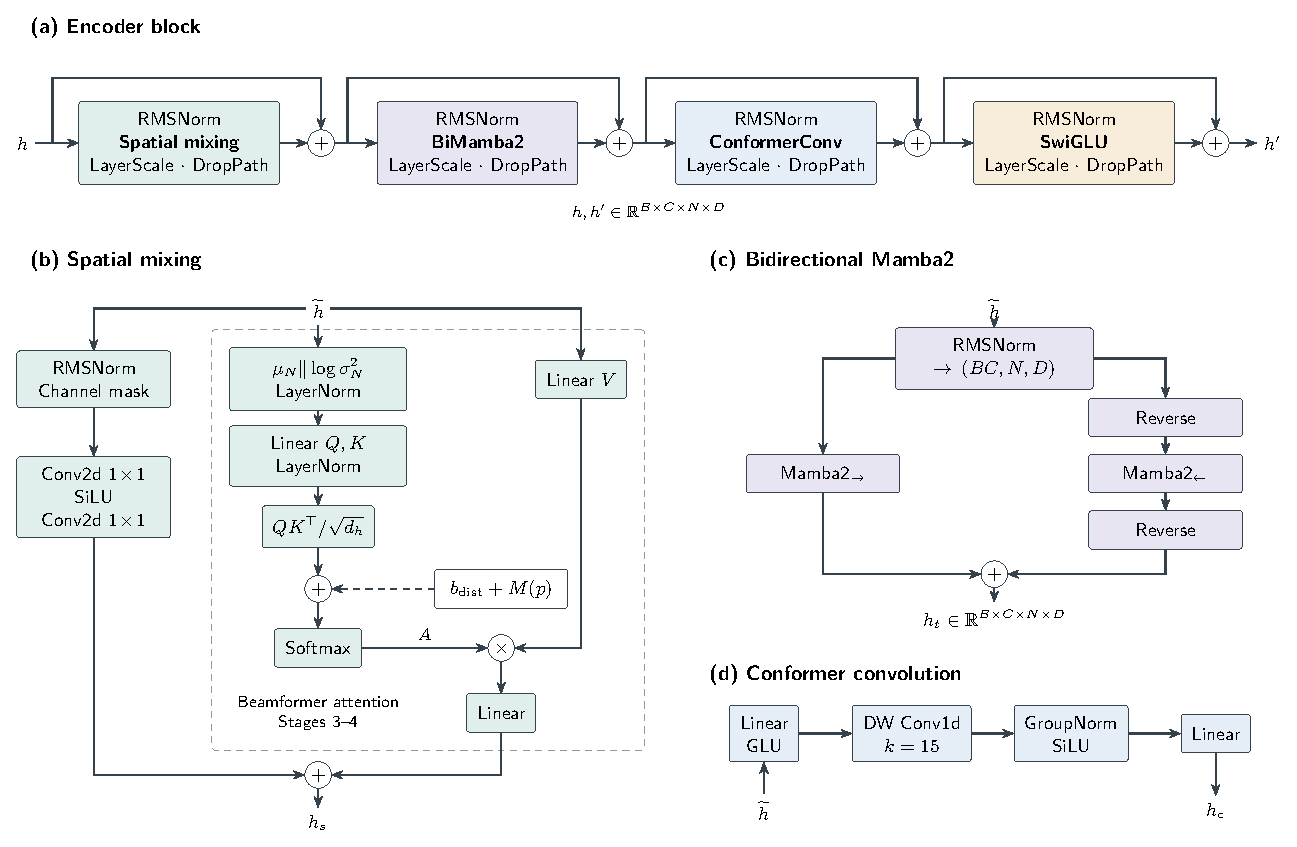
\includegraphics[width=\textwidth]{encoder_stage/encoder_stage.pdf}
    \caption{Encoder block and its constituent operations. Four pre-normalized
    residual branches perform spatial mixing, bidirectional Mamba2 processing,
    local temporal convolution, and a gated feed-forward transformation.
    Spatial attention is added to the convolutional spatial branch in stages
    three and four. $\widetilde h$ denotes a branch input after its outer
    normalization; $M(p)$ in the diagram is the additive channel-availability
    mask associated with the presence codes $a$ in the text.}
    \label{fig:encoder-block}
\end{figure*}

Every block preserves its input shape $B\times C\times N\times D$.
As shown in \cref{fig:encoder-block}, its four residual updates take the form
\begin{equation}
    U_r=U_{r-1}+\operatorname{DP}_{\rho}
    \bigl(\gamma_r\odot F_r(\RN_r(U_{r-1}))\bigr),
    \label{eq:residual-block}
\end{equation}
for $r=1,\ldots,4$, with $F_r$ denoting spatial mixing, temporal Mamba2,
Conformer convolution, and SwiGLU, respectively. Each branch has its own
normalization parameters and feature-wise LayerScale vector
$\gamma_r\in\mathbb{R}^{D}$, initialized to $10^{-4}$.
During training, DropPath multiplies a branch by
$\xi/(1-\rho)$, with $\xi\sim\operatorname{Bernoulli}(1-\rho)$ independently
sampled per batch example and branch. The rate $\rho$ increases linearly
from zero to 0.15 over the ten blocks. Ordinary dropout is zero in the
reference configuration.

\paragraph{Convolutional spatial mixing.}
Let $U$ denote the input to the spatial module, already normalized by the
outer residual branch. SpatialConv applies an additional RMSNorm and masks
unavailable input channels:
\begin{equation}
    G_{bcnd}=m_{bc}\,[\RN(U_{bcn})]_d.
\end{equation}
At every temporal and feature index, two $1\times1$ convolutions mix the
channel axis:
\begin{equation}
    S^{\mathrm{conv}}_{b,:,n,d}
    =W_{c,2}\SiLU(W_{c,1}G_{b,:,n,d}),
    \label{eq:spatial-conv}
\end{equation}
where $W_{c,1},W_{c,2}\in\mathbb{R}^{C\times C}$.
This branch is present in all stages and uses a fixed channel ordering.

\paragraph{Montage-dependent attention bias.}
Coordinates $p_i$ are taken from the standard 10--20 montage for the mapped
channel names. We normalize them and compute angular distances:
\begin{align}
    u_i&=\frac{p_i}{\max(\|p_i\|_2,\varepsilon)},\\
    d_{ij}&=\arccos\!\left(\operatorname{clip}(u_i^\top u_j,-1,1)\right).
\end{align}
The distances are discretized into $K_d=16$ bins,
\begin{equation}
    \beta_{ij}=\operatorname{round}\!\left(
      \frac{(K_d-1)d_{ij}}{\max(\max_{r,s}d_{rs},\varepsilon)}
    \right),
    \label{eq:distance-bins}
\end{equation}
where the denominator is clamped from below by
$\varepsilon=10^{-8}$. The resulting integer indices are fixed buffers.
A learned table $E\in\mathbb{R}^{A\times K_d}$, initialized to zero,
defines the head-specific bias $b_{hij}=E_{h,\beta_{ij}}$.
This table is shared across the attention blocks of the encoder.

\paragraph{Statistics-conditioned spatial attention.}
Stages three and four add a beamformer-style attention branch to
\cref{eq:spatial-conv}. For each channel, queries and keys are conditioned on
statistics over the temporal tokens:
\begin{align}
    \mu_{bc}&=\frac{1}{N}\sum_{n=1}^{N}U_{bcn},\\
    v_{bc}&=\frac{1}{N}\sum_{n=1}^{N}(U_{bcn}-\mu_{bc})^{\odot2},\\
    \ell_{bc}&=\log\bigl(\max(v_{bc},\varepsilon)\bigr),\\
    s_{bc}&=\LN(\mu_{bc}\Vert\ell_{bc}).
    \label{eq:channel-statistics}
\end{align}
The maximum and logarithm are element-wise, with $\varepsilon=10^{-8}$.
Each of the eight heads has feature width $d_h=D/A$ and computes
\begin{align}
    q_{bhi}&=\LN(W_h^Qs_{bi}),\\
    k_{bhj}&=\LN(W_h^Ks_{bj}).
\end{align}
The spatial weights are
\begin{align}
    e_{bhij}&=q_{bhi}^{\top}k_{bhj}/\sqrt{d_h}+b_{hij},\\
    A_{bhij}&=\frac{m_{bj}\exp(e_{bhij})}
                      {\sum_r m_{br}\exp(e_{bhir})}.
    \label{eq:spatial-attention}
\end{align}
Values retain the temporal axis: $v_{bhjn}=W_h^VU_{bjn}$.
For each time index, the attention output is
\begin{equation}
    S^{\mathrm{attn}}_{bin}
      =W_O\!\left(\mathop{\Vert}_{h=1}^{A}
        \sum_j A_{bhij}v_{bhjn}\right).
\end{equation}
A single spatial weight matrix per window and head is therefore reused
across all temporal tokens. The spatial residual branch receives
$S^{\mathrm{conv}}$ in stages one and two and
$S^{\mathrm{conv}}+S^{\mathrm{attn}}$ in stages three and four.
The geometric bias informs attention about relative electrode locations;
the channel embeddings and convolutional mixing nevertheless retain a fixed
channel indexing, so this construction does not imply arbitrary-montage
or channel-permutation invariance.

\paragraph{Bidirectional temporal state-space processing.}
Temporal dependencies are modeled with two independently parameterized
Mamba2 modules~\cite{dao2024mamba2}. After an internal RMSNorm, the tensor
is reshaped to $(BC,N,D)$, treating each electrode as a separate sequence.
Writing $R$ for reversal along the token axis and $\bar U=\RN(U)$, the
bidirectional output is
\begin{equation}
    F_{\mathrm{temp}}(U)
      =\mathcal{M}_{\rightarrow}(\bar U)
       +R\!\left[\mathcal{M}_{\leftarrow}(R[\bar U])\right].
    \label{eq:bimamba}
\end{equation}
Reversing the backward output restores the original token alignment before
summation. Each Mamba2 module uses state dimension 128, expansion factor two,
local convolution width four, and head dimension 64. This module mixes
information across time within each electrode; interactions between
electrodes are provided by the spatial branch.

For completeness, the selective state-space core of a single Mamba2 head
can be expressed in recurrent form as
\begin{align}
    S_n&=\eta_n S_{n-1}+b_n v_n^\top,\\
    o_n&=S_n^\top c_n+d\,v_n,
    \label{eq:mamba-state}
\end{align}
where $S_n\in\mathbb{R}^{128\times64}$, $v_n\in\mathbb{R}^{64}$,
and $b_n,c_n\in\mathbb{R}^{128}$. The scalar transition $\eta_n$ and the
input and readout vectors depend on the input; $b_n$ includes the input
scaling from discretization, and $d$ is a learned direct-path coefficient.
This scalar-identity transition is the structured state-space component of
Mamba2~\cite{dao2024mamba2}. The complete module also includes its input
projections, local convolution, gating, normalization, and output projection.
\Cref{eq:bimamba} combines two such complete modules in opposite directions.

\paragraph{Local temporal convolution and gated feed-forward mapping.}
The Conformer branch supplements the state-space module with a local
convolution. A linear map expands $U$ from $D$ to $4D$ features and splits
it into $a,b\in\mathbb{R}^{2D}$. The gated features are
$v=a\odot\sigma(b)$, where $\sigma$ is the sigmoid. A depthwise temporal
convolution of kernel size 15, with padding that preserves $N$, is followed
by single-group GroupNorm, SiLU, and a projection back to $D$:
\begin{equation}
    F_{\mathrm{conv}}(U)
      =W_2\SiLU\!\left(\operatorname{GN}
        (\operatorname{DWConv}_{15}(v))\right).
\end{equation}
Finally, the feature-wise SwiGLU branch is
\begin{equation}
    F_{\mathrm{ffn}}(U)=W_3
      \bigl(\SiLU(W_1U)\odot W_2U\bigr).
\end{equation}
Its hidden width is $\lfloor8D/3\rfloor$ rounded upward to the nearest
multiple of 64. All four operations are wrapped by the residual update
in \cref{eq:residual-block}.

\subsection{Training Pipeline Overview}
\label{sec:training}

\begin{figure*}[t]
    \centering
    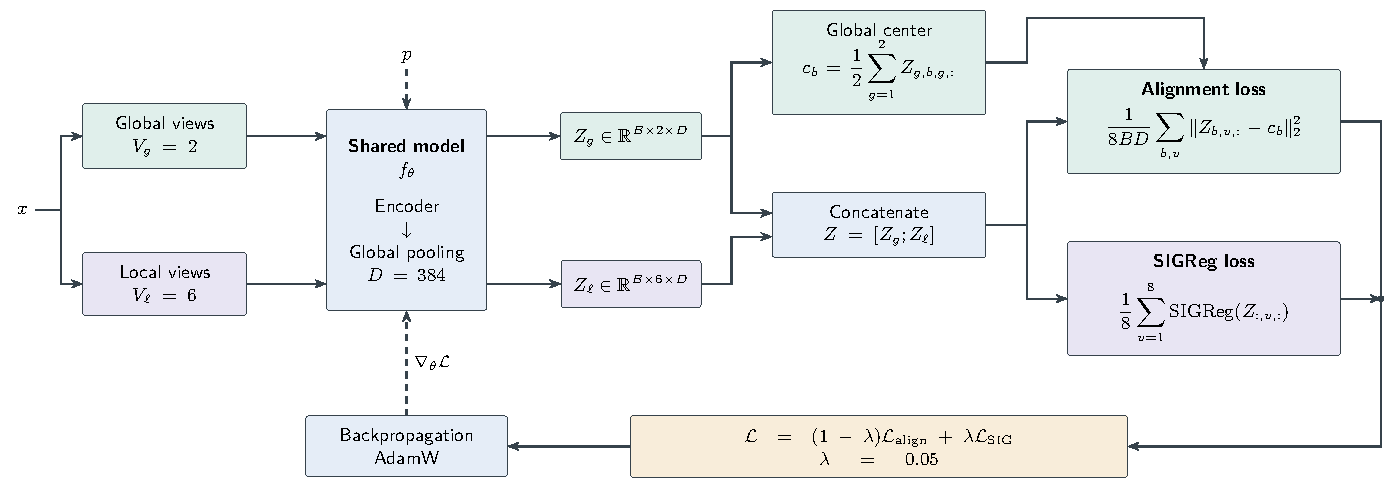
\includegraphics[width=\textwidth]{training_pipeline/training_pipeline.pdf}
    \caption{Multiview LeJEPA training. Two global and six local views are
    encoded by the same EEGFM parameters. All view embeddings are aligned
    with the mean of the global embeddings of their source window. SIGReg
    is evaluated across the batch separately for each view and then averaged.
    The weighted loss updates the complete encoder and global readout.
    The global center remains differentiable.}
    \label{fig:training-pipeline}
\end{figure*}

\paragraph{Multiview joint-embedding learning.}
LeJEPA combines a joint-embedding agreement objective with Sketched
Isotropic Gaussian Regularization~\cite{balestriero2025lejepa}, abbreviated SIGReg.
Our EEG adaptation applies both terms directly to the global readout
in \cref{eq:global-embedding}. It uses a single shared encoder, with no
separate teacher, stop-gradient target, predictor network, or additional
projection head. The active training path does not reconstruct EEG signals.

For each source window $X_b$, the data loader supplies $V_g=2$ global views
and $V_\ell=6$ local views. We denote their union by
$x_b^{(v)}=\mathcal{T}_v(X_b)$, $v=1,\ldots,V$, where $V=V_g+V_\ell=8$ and
the first $V_g$ indices designate the global views.
The augmentation configuration includes additive noise, global and
channel-wise amplitude scaling, temporal shifts, and temporal, frequency,
and spatial masking. The same presence codes $a_b$ accompany all views of
a window. Each view is passed through the same model:
\begin{equation}
    y_b^{(v)}=g_\theta(x_b^{(v)},a_b;P)
      \in\mathbb{R}^{D_z}.
\end{equation}
Here $g_\theta$ denotes the global component of $f_\theta$.
Stacking these outputs yields tensors of shape $B\times V_g\times D_z$
and $B\times V_\ell\times D_z$, as shown in \cref{fig:training-pipeline}.

\paragraph{Alignment with the global-view center.}
The target for every view of window $b$ is the mean of its global embeddings,
\begin{equation}
    c_b=\frac{1}{V_g}\sum_{v=1}^{V_g}y_b^{(v)}.
    \label{eq:global-center}
\end{equation}
Both global and local embeddings contribute to the alignment loss,
\begin{equation}
    \mathcal{L}_{\mathrm{align}}
      =\frac{1}{BVD_z}\sum_{b=1}^{B}\sum_{v=1}^{V}
         \|y_b^{(v)}-c_b\|_2^2.
    \label{eq:alignment}
\end{equation}
The factor $D_z^{-1}$ matches averaging over features in the implementation.
Gradients propagate through both the individual embeddings and the center
$c_b$. Alignment alone admits a constant representation, motivating the
additional distributional constraint.

\paragraph{Sketched isotropic Gaussian regularization.}
At each optimization step, we sample $K=256$ unit directions
$u_k=\omega_k/\|\omega_k\|_2$, with
$\omega_k\sim\mathcal{N}(0,I_{D_z})$.
For a fixed view $v$, the one-dimensional projections
$s_{bvk}=u_k^\top y_b^{(v)}$ define an empirical characteristic function
\begin{equation}
    \widehat\varphi_{vk}(t)
       =\frac{1}{B}\sum_{b=1}^{B}\exp(\mathrm{i}t s_{bvk}).
    \label{eq:empirical-cf}
\end{equation}
The target is the characteristic function of a standard normal variable,
$\varphi_0(t)=\exp(-t^2/2)$. Define
\begin{equation}
    e_{vk}(t)=
      |\widehat\varphi_{vk}(t)-\varphi_0(t)|^2\varphi_0(t).
\end{equation}
The implemented per-view regularizer approximates
\begin{equation}
    \mathcal{R}_v=\frac{B}{K}\sum_{k=1}^{K}
       \int_{-5}^{5}e_{vk}(t)\,\mathrm{d}t
    \label{eq:sigreg-integral}
\end{equation}
using the trapezoidal rule on $J=17$ equally spaced points
$t_j=-5+10j/(J-1)$, $j=0,\ldots,J-1$:
\begin{equation}
    \mathcal{R}_v\approx\frac{B\Delta t}{2K}
      \sum_{k=1}^{K}\sum_{j=0}^{J-2}
      \bigl[e_{vk}(t_j)+e_{vk}(t_{j+1})\bigr],
    \label{eq:sigreg-discrete}
\end{equation}
where $\Delta t=10/(J-1)$.
The complex discrepancy is evaluated through its real and imaginary parts,
\begin{equation}
    |\widehat\varphi-\varphi_0|^2
      =(\Re\widehat\varphi-\varphi_0)^2
        +(\Im\widehat\varphi)^2.
\end{equation}
This operates on the unnormalized embeddings, so the unit-variance target
also constrains their scale. The final regularizer is
\begin{equation}
    \mathcal{L}_{\mathrm{SIG}}=\frac{1}{V}\sum_{v=1}^{V}\mathcal{R}_v.
    \label{eq:sigreg-views}
\end{equation}
Thus, views are not pooled together as independent samples for SIGReg.
The same random directions are reused across views within a step by seeding
the sampler with the global step index. If distributed training is
initialized, characteristic-function sums and sample counts are aggregated
across workers; $B$ in \cref{eq:empirical-cf,eq:sigreg-integral,eq:sigreg-discrete}
then denotes the aggregated batch size. The regularizer is evaluated in
float32 when embeddings are produced in reduced precision.

\paragraph{Objective and optimization.}
The complete objective is
\begin{equation}
    \mathcal{L}=(1-\lambda)\mathcal{L}_{\mathrm{align}}
                   +\lambda\mathcal{L}_{\mathrm{SIG}},
    \qquad\lambda=0.05.
    \label{eq:total-objective}
\end{equation}
The reference configuration selects TUEG windows with mapped channels and
enables normalization in the data loader. The optimizer is AdamW with
initial learning rate $10^{-4}$, momentum coefficients $(0.9,0.95)$,
and weight decay 0.05 on the designated parameter group. Biases,
normalization parameters, embeddings, learned queries, LayerScale vectors,
and the spatial bias table are excluded from weight decay by the model's
parameter-group rules. The total gradient norm is clipped at one.
A cosine learning-rate schedule is stepped after every optimizer update,
with a 10,000-step horizon and minimum learning rate $10^{-5}$.
The configuration uses batches of 16, bfloat16 autocasting, and gradient
checkpointing within encoder blocks. It specifies 20 epochs, capped at
500 training batches and 100 validation batches per epoch.

The objective encourages agreement under the selected view transformations
while penalizing departures from the Gaussian projection target. Neither
term explicitly removes subject identity, acquisition-related information,
or artifacts shared across views. Whether the resulting representations
retain useful information under montage changes must therefore be
established by downstream evaluations and ablations.

\balance
\section{Results}

\subsection{Linear Probing}

Linear probing assesses how readily task labels can be decoded from a
pretrained representation without adapting the backbone. Each foundation
model is frozen and used in evaluation mode to extract features $H=f_\theta(X)$.
Since output shapes differ across models, all non-batch dimensions are
flattened into one feature vector per example:
\begin{equation}
    U=\operatorname{Flatten}_{\mathrm{non\text{-}batch}}(H)
    \in\mathbb{R}^{B\times F}.
\end{equation}
Thus, outputs of shape $B\times C\times D$ or $B\times C\times L\times D$
yield $F=CD$ or $F=CLD$, respectively, preserving channel and token features
without pooling. Each backbone has its own probe and a fixed feature
dimension within the evaluation setting. Only the linear classifier is
trained on labeled training examples, using either a single affine layer
with a classification loss or a linear support vector machine (SVM).
Performance on held-out data measures the linear accessibility of
task-related information in the frozen features. This limits the contribution
of a flexible downstream classifier, while preserving the representations'
full feature structure.

\subsection{Ablation study on }


\section{Discussion and Conclusion}




\begingroup
\small
\raggedright
\bibliographystyle{plain}
\IfFileExists{references.bib}{\bibliography{references}}{\bibliography{report/references}}
\endgroup
\end{document}
